\documentclass[11pt, a4paper]{article}
\usepackage{pdfpages}
\usepackage{parallel}
\usepackage[T2A]{fontenc}
\usepackage{ucs}
\usepackage[utf8x]{inputenc}
\usepackage[polish,english,russian]{babel}
\usepackage{hyperref}
\usepackage{rotating}
\usepackage[inner=2cm,top=1.8cm,outer=2cm,bottom=2.3cm,nohead]{geometry}
\usepackage{listings}
\usepackage{graphicx}
\usepackage{wrapfig}
\usepackage{longtable}
\usepackage{indentfirst}
\usepackage{array}
\usepackage{tikzsymbols}
\usepackage{soul}
\usepackage[ruled,vlined]{algorithm2e}
%\counterwithout{figure}{section} 

\usepackage{url}
\makeatletter
\g@addto@macro{\UrlBreaks}{\UrlOrds}
\makeatother

\newcolumntype{P}[1]{>{\raggedright\arraybackslash}p{#1}}
\frenchspacing
\usepackage{fixltx2e} %text sub- and superscripts
\usepackage{icomma} % коскі ў матэматычным рэжыме
\PreloadUnicodePage{4}

\newcommand{\longpage}{\enlargethispage{\baselineskip}}
\newcommand{\shortpage}{\enlargethispage{-\baselineskip}}

\def\switchlang#1{\expandafter\csname switchlang#1\endcsname}
\def\switchlangbe{
\let\saverefname=\refname%
\def\refname{Літаратура}%
\def\figurename{Іл.}%
}
\def\switchlangen{
\let\saverefname=\refname%
\def\refname{References}%
\def\figurename{Fig.}%
}
\def\switchlangru{
\let\saverefname=\refname%
\let\savefigurename=\figurename%
\def\refname{Литература}%
\def\figurename{Рис.}%
}

\hyphenation{admi-ni-stra-tive}
\hyphenation{ex-pe-ri-ence}
\hyphenation{fle-xi-bi-li-ty}
\hyphenation{Py-thon}
\hyphenation{ma-the-ma-ti-cal}
\hyphenation{re-ported}
\hyphenation{imp-le-menta-tions}
\hyphenation{pro-vides}
\hyphenation{en-gi-neering}
\hyphenation{com-pa-ti-bi-li-ty}
\hyphenation{im-pos-sible}
\hyphenation{desk-top}
\hyphenation{elec-tro-nic}
\hyphenation{com-pa-ny}
\hyphenation{de-ve-lop-ment}
\hyphenation{de-ve-loping}
\hyphenation{de-ve-lop}
\hyphenation{da-ta-ba-se}
\hyphenation{plat-forms}
\hyphenation{or-ga-ni-za-tion}
\hyphenation{pro-gramming}
\hyphenation{in-stru-ments}
\hyphenation{Li-nux}
\hyphenation{sour-ce}
\hyphenation{en-vi-ron-ment}
\hyphenation{Te-le-pathy}
\hyphenation{Li-nux-ov-ka}
\hyphenation{Open-BSD}
\hyphenation{Free-BSD}
\hyphenation{men-ti-on-ed}
\hyphenation{app-li-ca-tion}

\def\progref!#1!{\texttt{#1}}
\renewcommand{\arraystretch}{2} %Іначай формулы ў матрыцы зліпаюцца з лініямі
\usepackage{array}

\def\interview #1 (#2), #3, #4, #5\par{

\section[#1, #3, #4]{#1 -- #3, #4}
\def\qname{LVEE}
\def\aname{#1}
\def\q ##1\par{{\noindent \bf \qname: ##1 }\par}
\def\a{{\noindent \bf \aname: } \def\qname{L}\def\aname{#2}}
}

\def\interview* #1 (#2), #3, #4, #5\par{

\section*{#1\\{\small\rm #3, #4. #5}}
\ifx\ParallelWhichBox\undefined%
    \addcontentsline{toc}{section}{#1, #3, #4}%
\else%
\ifnum\ParallelWhichBox=0%
    \addcontentsline{toc}{section}{#1, #3, #4}%
\fi\fi%

\def\qname{LVEE}
\def\aname{#1}
\def\q ##1\par{{\noindent \bf \qname: ##1 }\par}
\def\a{{\noindent \bf \aname: } \def\qname{L}\def\aname{#2}}
}

\newcommand{\interviewfooter}[1]{
\vskip 1em
\noindent \textit{#1}
}

\switchlang{en}
\begin{document}

\title{1983 "--- Microsoft Green Eyed Mouse}
\date{}
\maketitle
\selectlanguage{english}

Microsoft's first mouse was released in 1983 and was also the first product from its hardware division, which the company opened a year earlier. Because of the two green buttons, this model is known as the ``green-eyed mouse''.

Since Microsoft at that time did not have enough experience in the hardware development and manufacture, the real manufacturer of the mouse was the Japanese company Alps -- the manufacturer of the first Japanese mouse, MZ-1X10, introduced in the same 1983.

\begin{figure}[h]
   \centering
    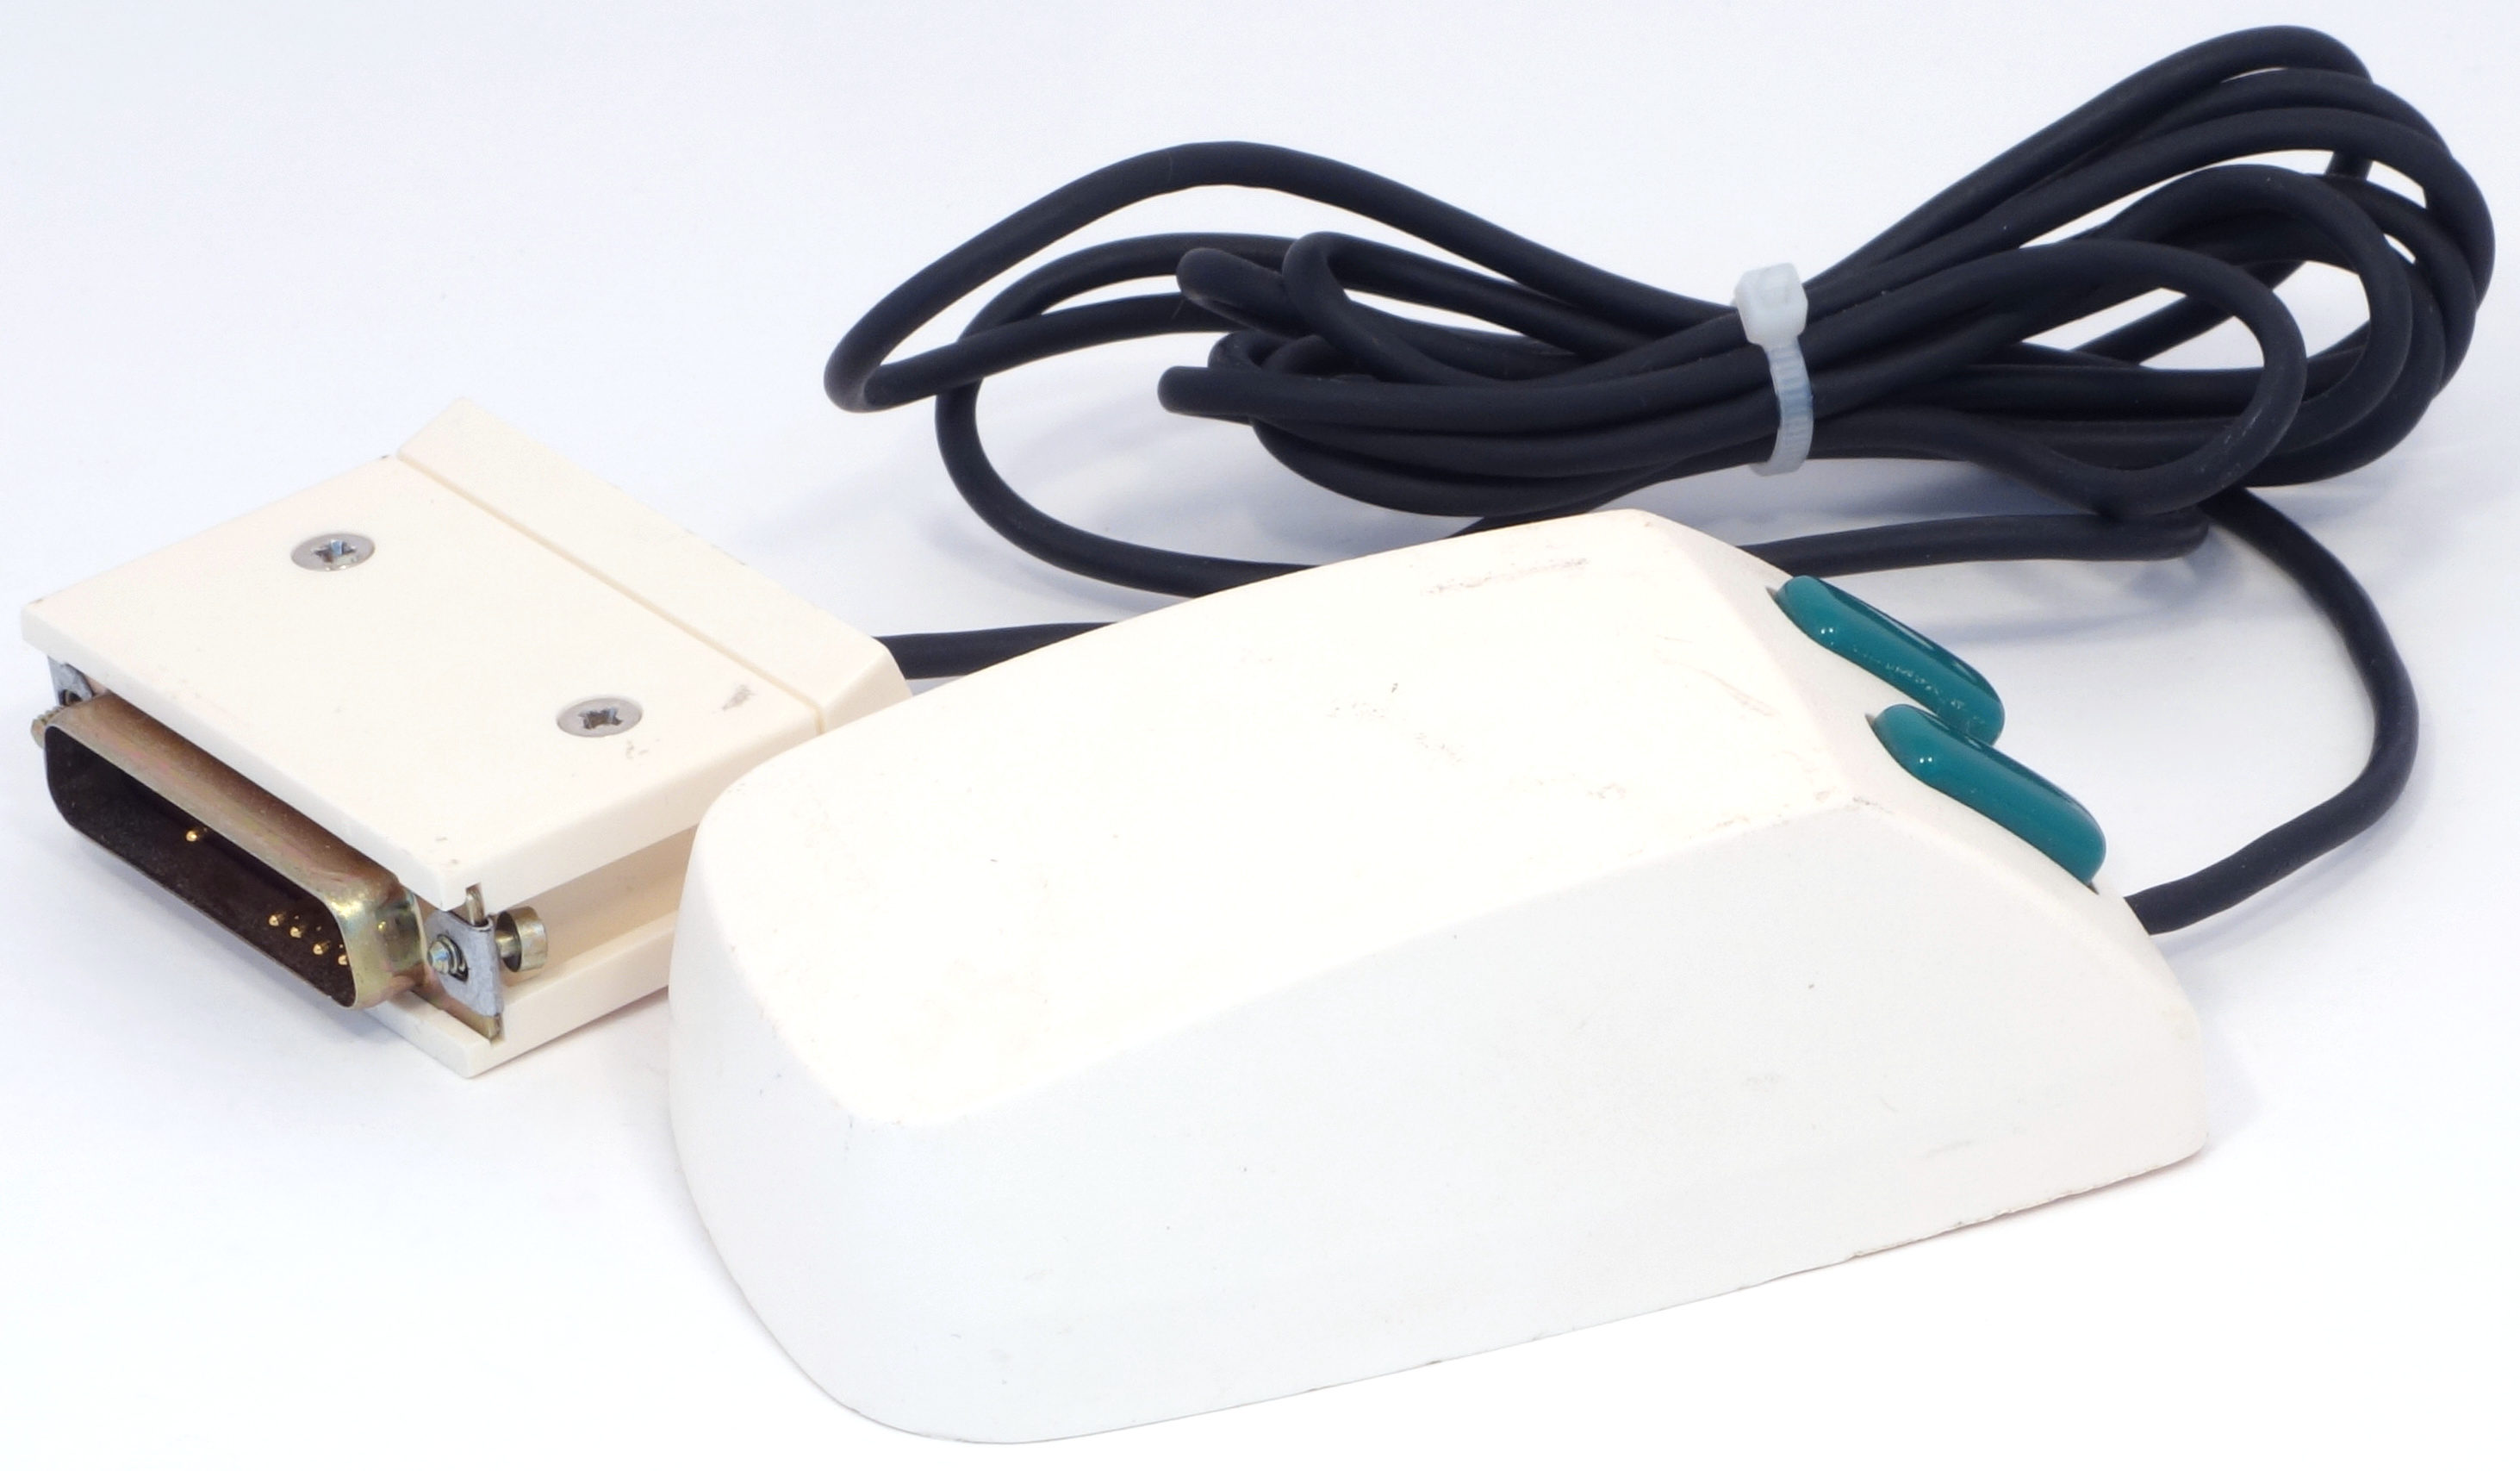
\includegraphics[scale=0.6]{1983_microsoft_green_eyed_mouse/pic_30.jpg}
    \caption{Microsoft Green Eyed Mouse}
    \label{fig:MicrosoftGreenEyedPic}
\end{figure}

Technically, Microsoft's first mouse and the MZ-1X10 have a lot in common. However, the body of the MZ-1X10 mouse is a cuboid with slightly rounded edges and a pair of rectangular buttons on the upper side of the body, while the body of the Microsoft mouse has a more complex shape, and the buttons are shifted to the sloping front side. (fig.  \ref{fig:MicrosoftGreenEyedPic}).

\begin{figure}[h]
    \centering
    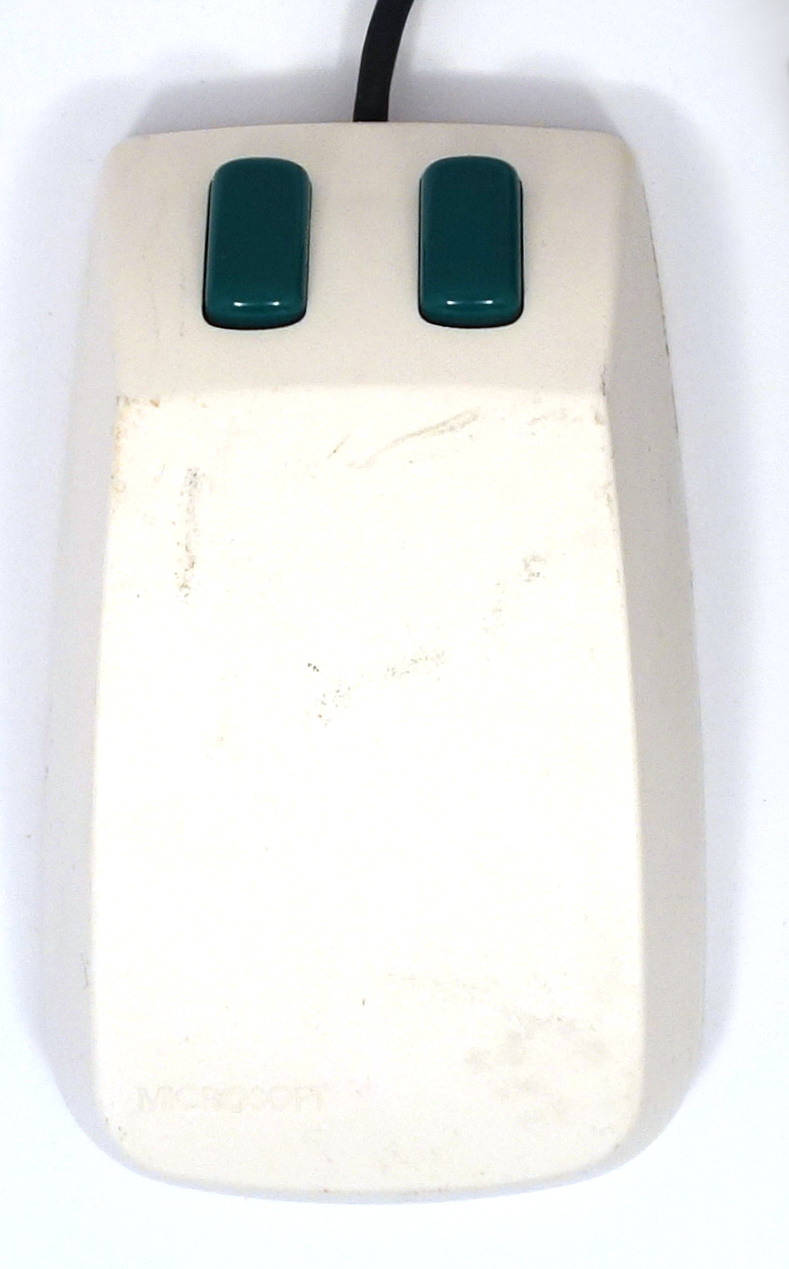
\includegraphics[scale=0.6]{1983_microsoft_green_eyed_mouse/top_60.jpg}
    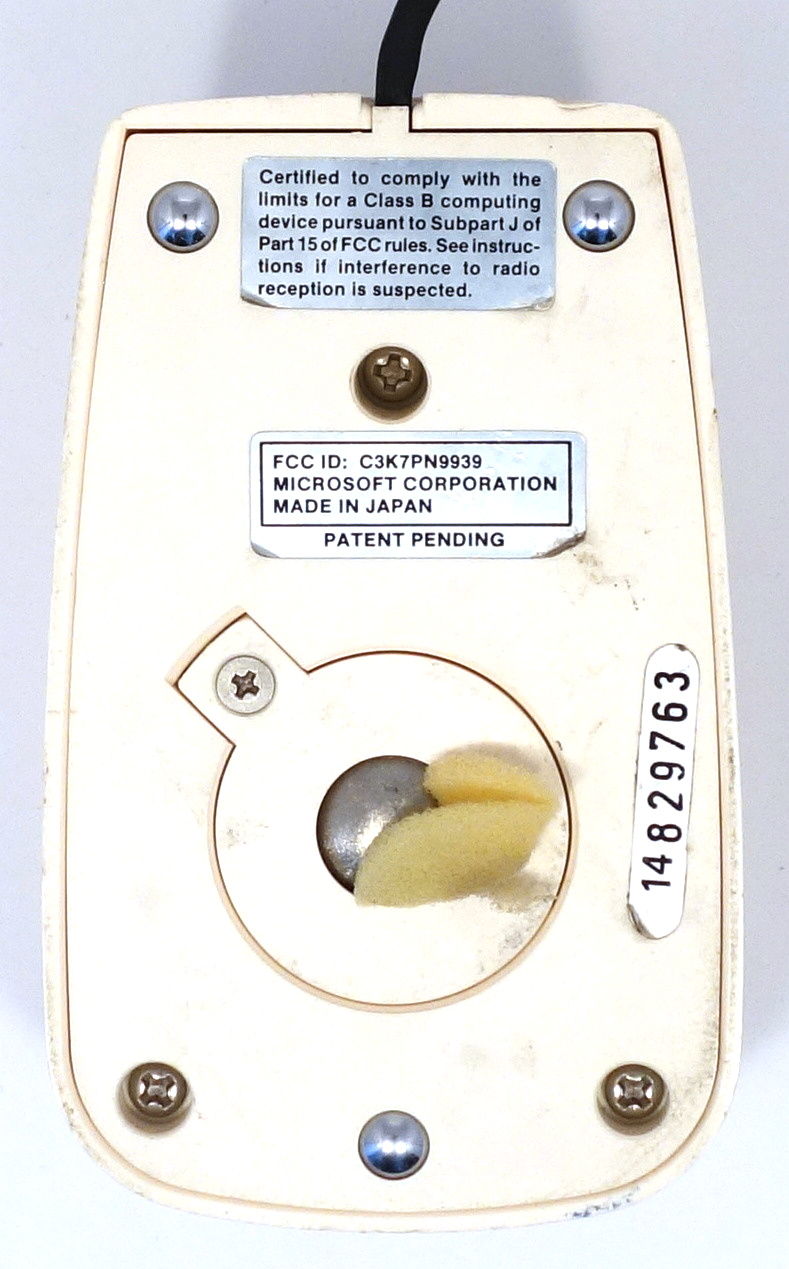
\includegraphics[scale=0.6]{1983_microsoft_green_eyed_mouse/bottom_60.jpg}
    \caption{Microsoft Green Eyed Mouse, top and bottom views}
    \label{fig:MicrosoftGreenEyedTopAndBottom}
\end{figure}

Clearly, Microsoft placed a lot of importance on the design of their mouse. The light cream-colored case is made in a minimalist style, the only elements are two contrasting green buttons and a barely noticeable company name at the edge of the body closest to the user (fig. \ref{fig:MicrosoftGreenEyedTopAndBottom}). Motion is detected by a heavy steel ball located towards the back of the mouse, and three small, smooth-polished balls act as feet to minimize friction. Also, a removable ring is provided in the bottom of the case, which allows you to remove the ball and get rid of the collected debris; however, the snap ring option has not yet been invented, so it must be unscrewed with a screwdriver.

\begin{figure}[h]
    \centering
    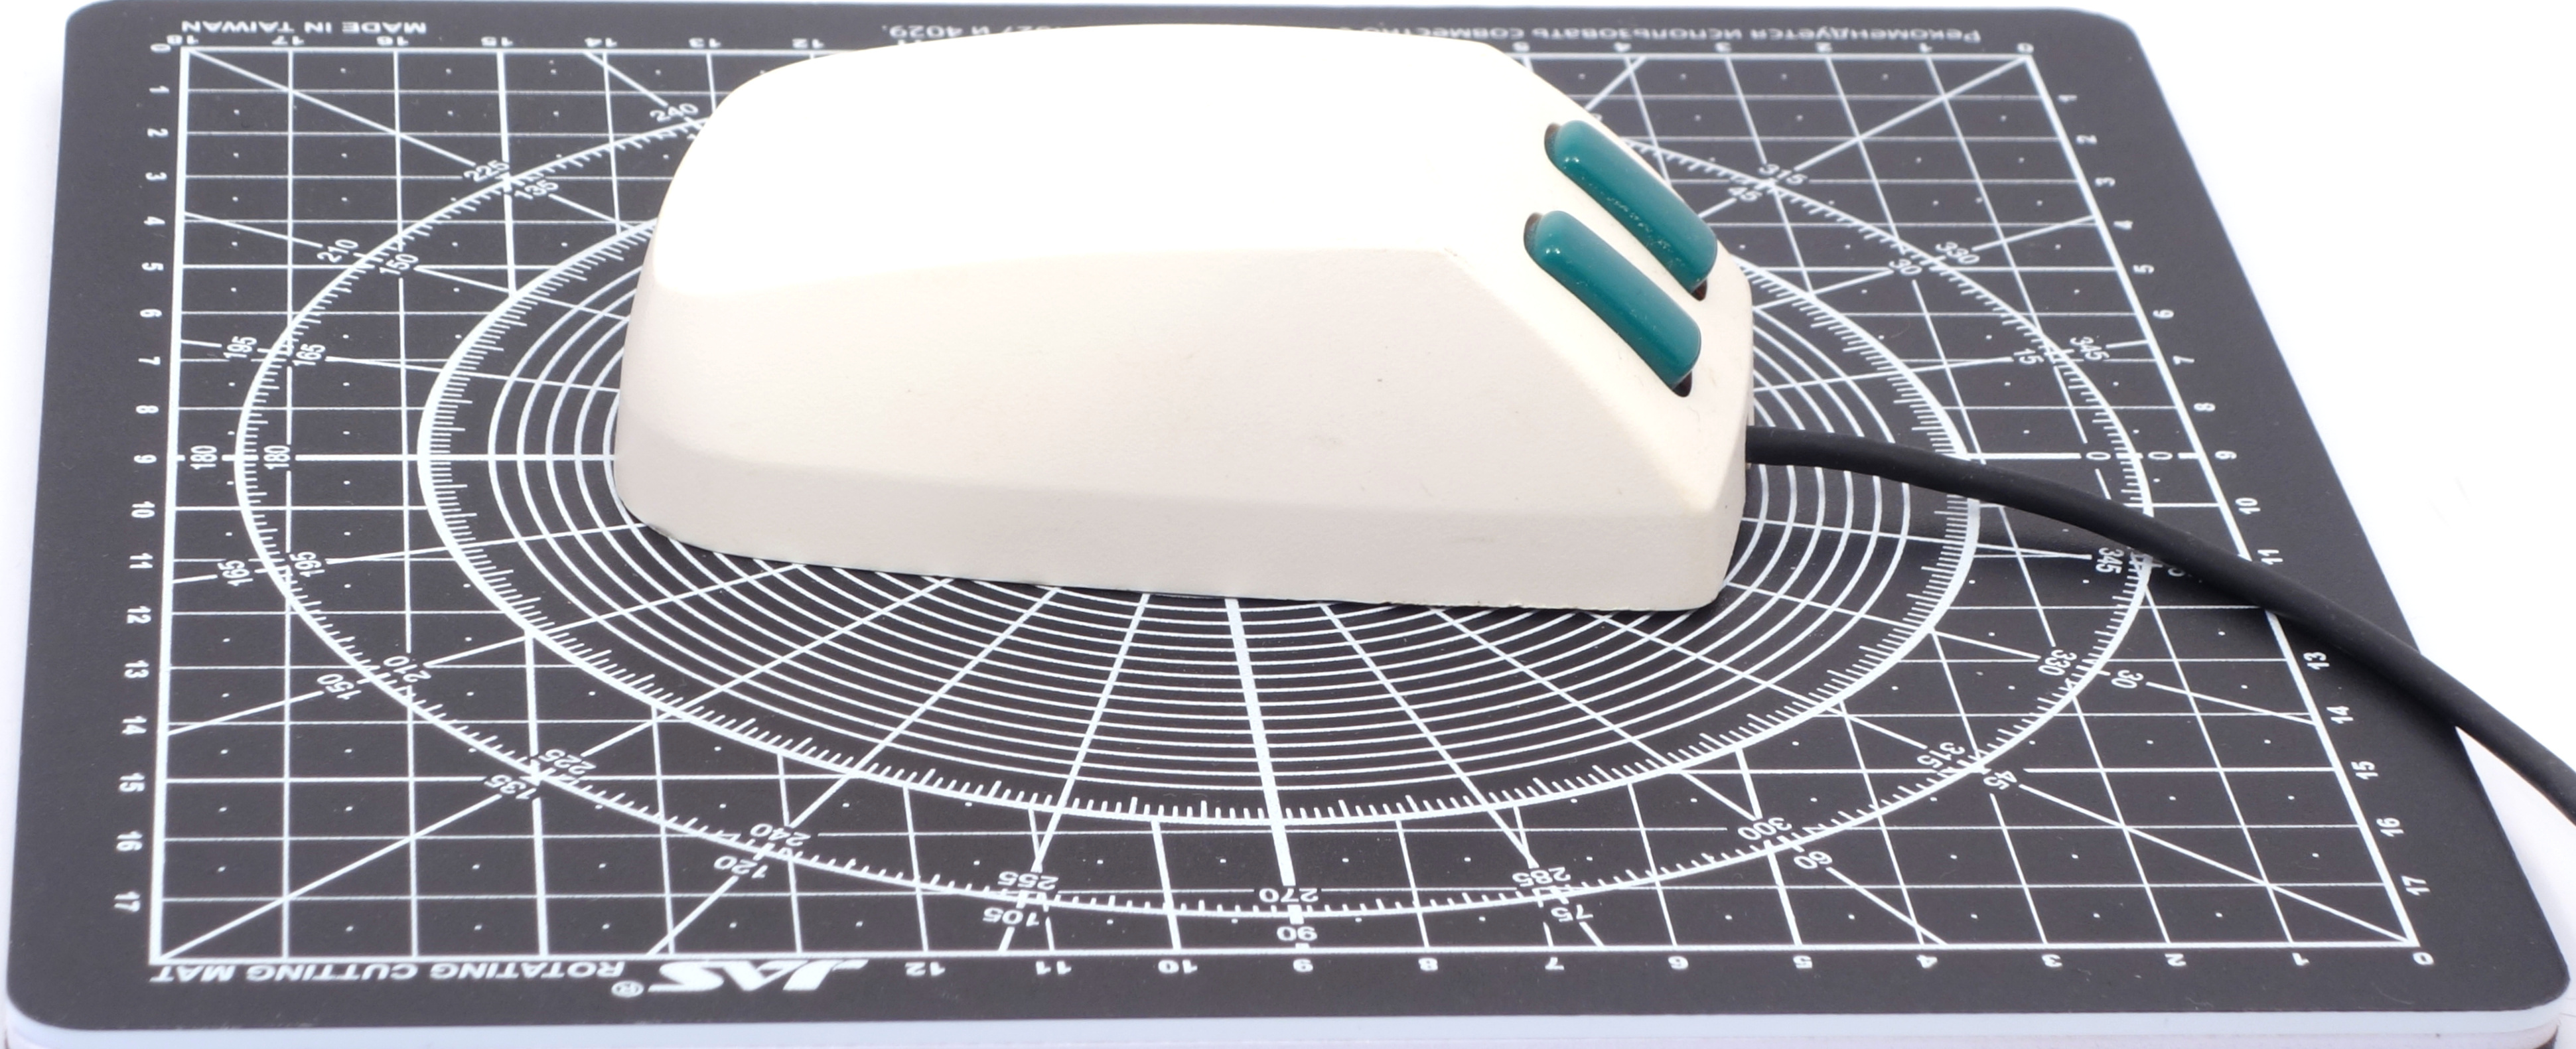
\includegraphics[scale=0.5]{1983_microsoft_green_eyed_mouse/size_30.jpg}
    \caption{Microsoft Green Eyed Mouse on a graduated pad with a grid step of 1~cm}
    \label{fig:MicrosoftGreenEyedSize}
\end{figure}

Despite the small size of the mouse (fig. \ref{fig:MicrosoftGreenEyedSize}), it is quite heavy. Clearly, Microsoft's focus on body shape was more or less beneficial to ergonomics. Compared to its closest relative, the MZ-1X10 mouse, it allows the palm and fingers to be placed in a more natural position. (fig. \ref{fig:MicrosoftGreenEyedHand}).

\begin{figure}[h]
    \centering
    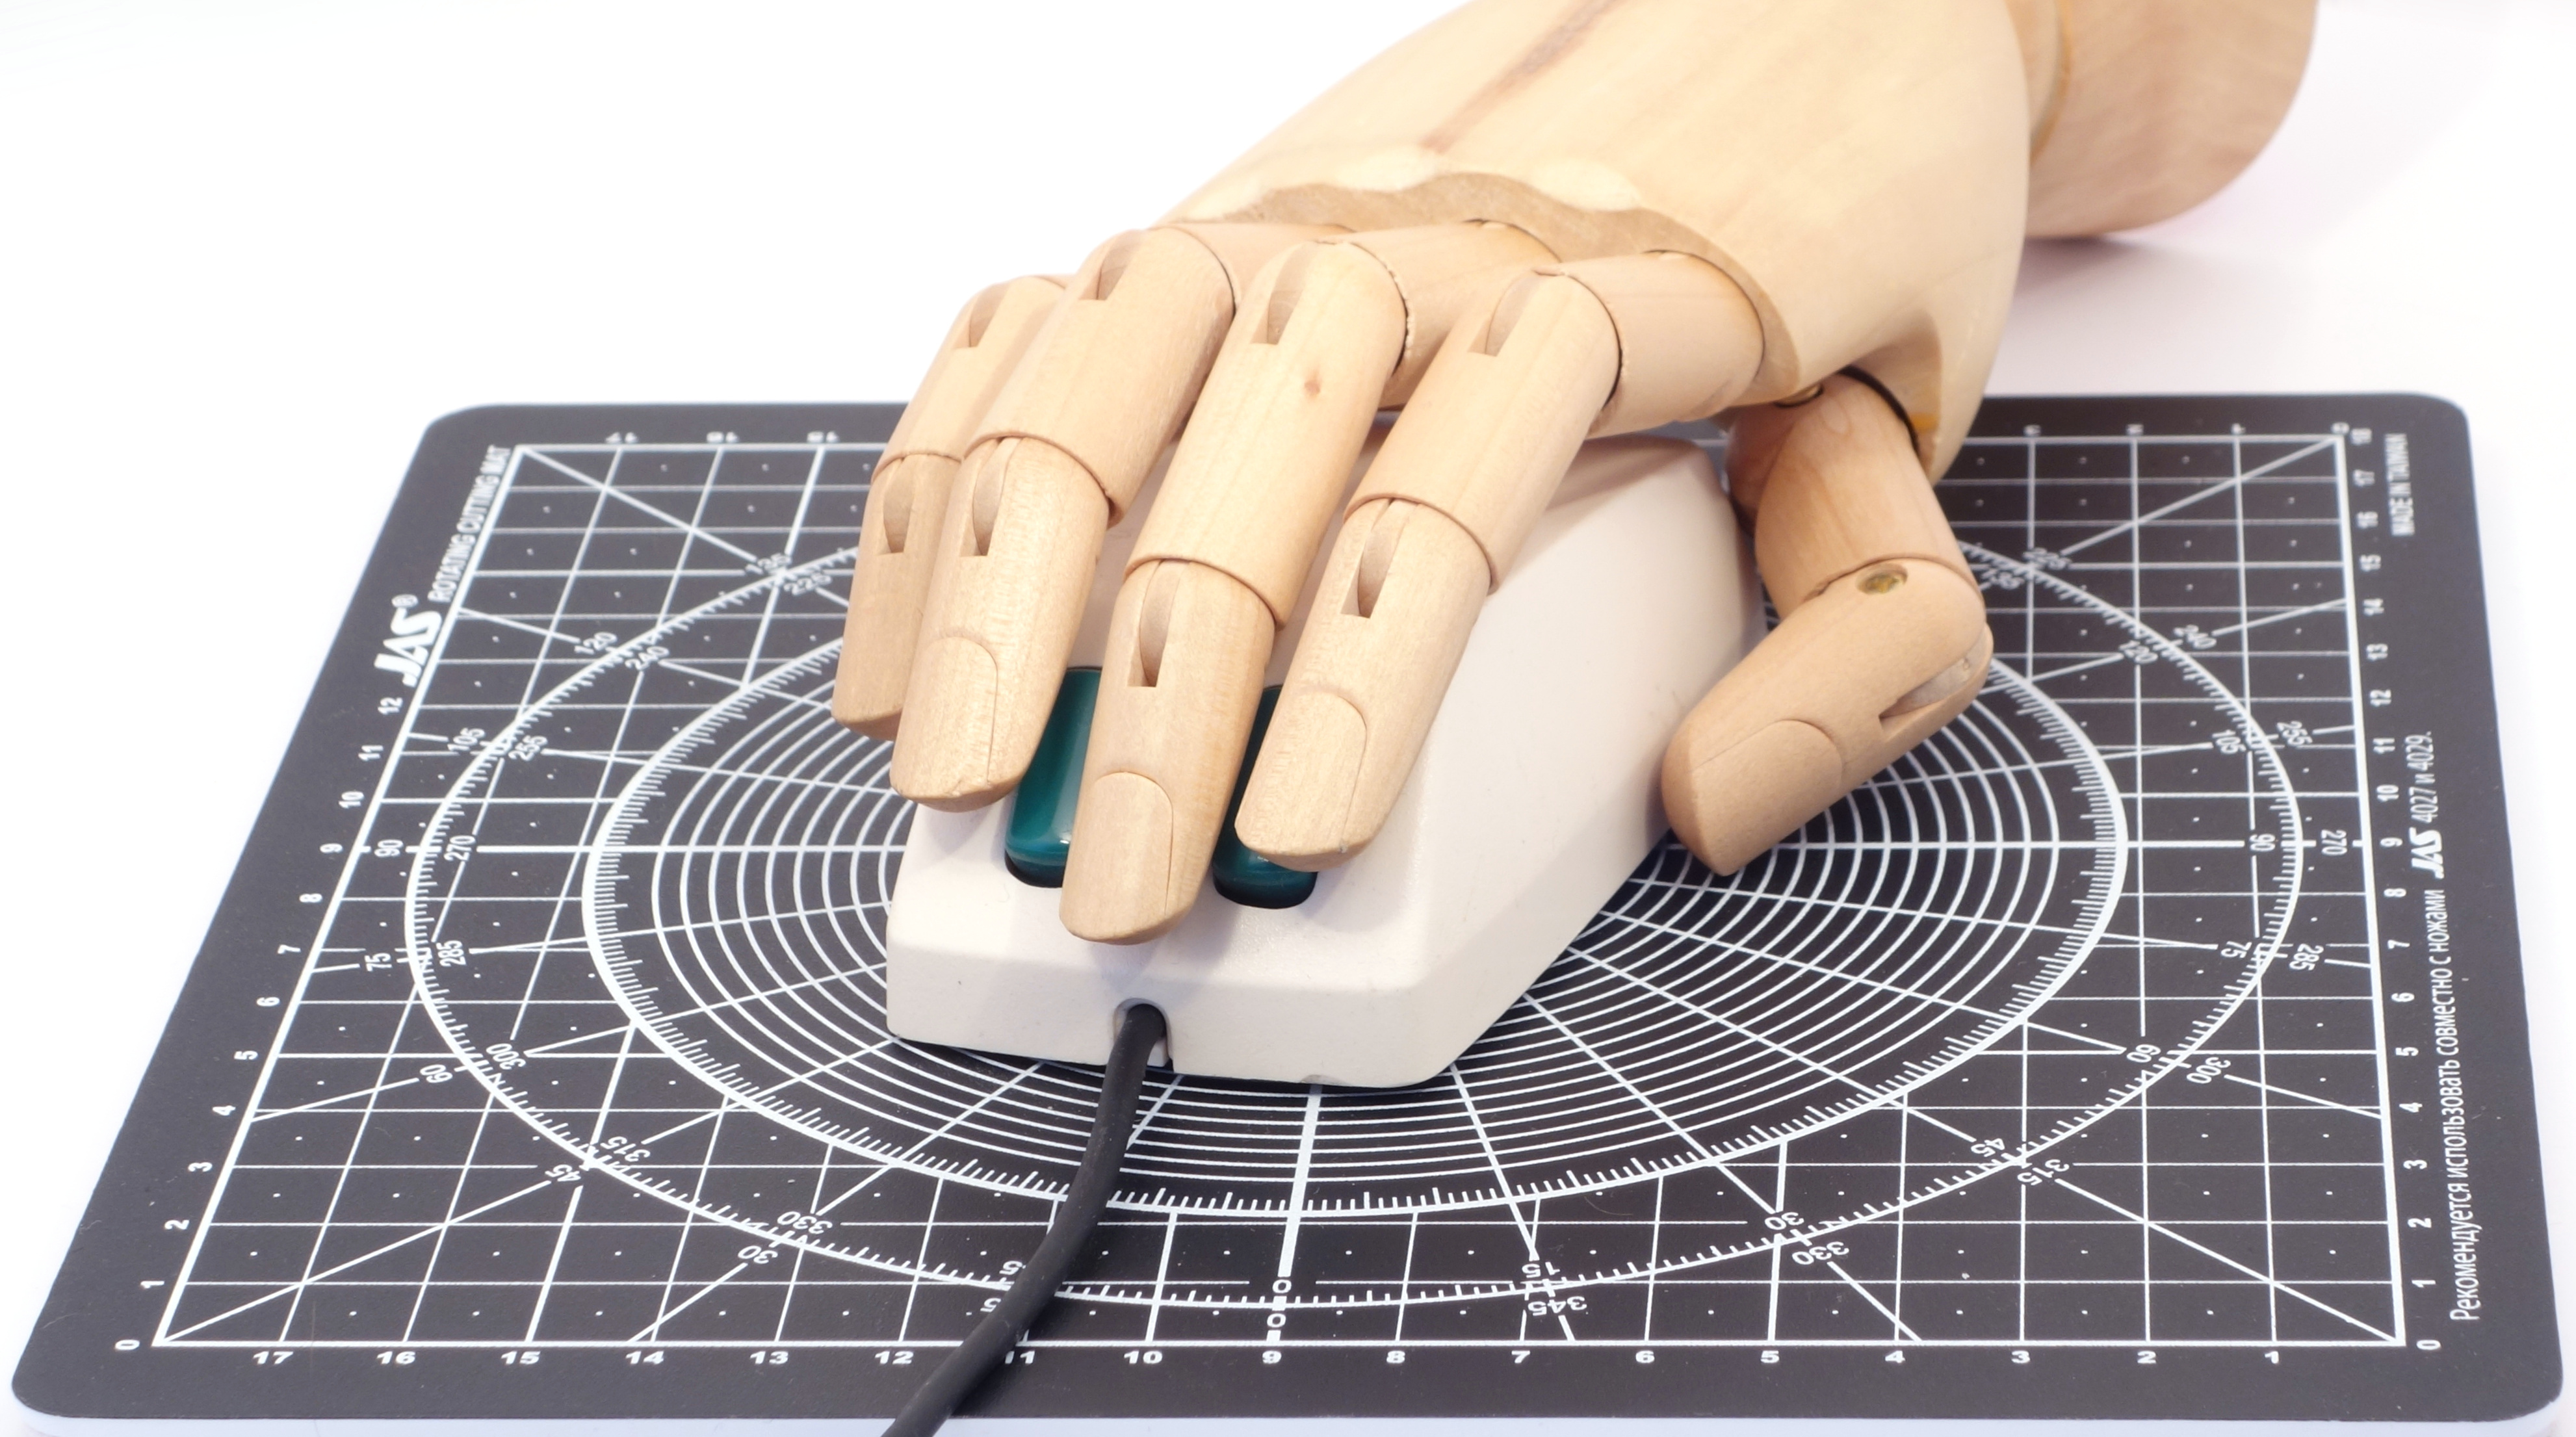
\includegraphics[scale=0.5]{1983_microsoft_green_eyed_mouse/hand_30.jpg}
    \caption{Microsoft Green Eyed Mouse with a human hand model}
    \label{fig:MicrosoftGreenEyedHand}
\end{figure}

Early versions of the Microsoft mouse had a bus interface and were equipped with a special adapter board. Later versions appeared with a serial interface and a 25 or 9-pin connector \cite{mouses}. Mouse resolution was only 100 DPI \cite{review}.

The internal structure of the mouse can be seen in fig. \ref{fig:MicrosoftGreenEyedInside}. The mouse uses closed contact encoders. When compared with the MZ-1X10 mouse, the technical design is almost identical: the differences come down to the configuration of the printed circuit board and are obviously caused by the front placement of the buttons.

 \begin{figure}[h]
    \centering
    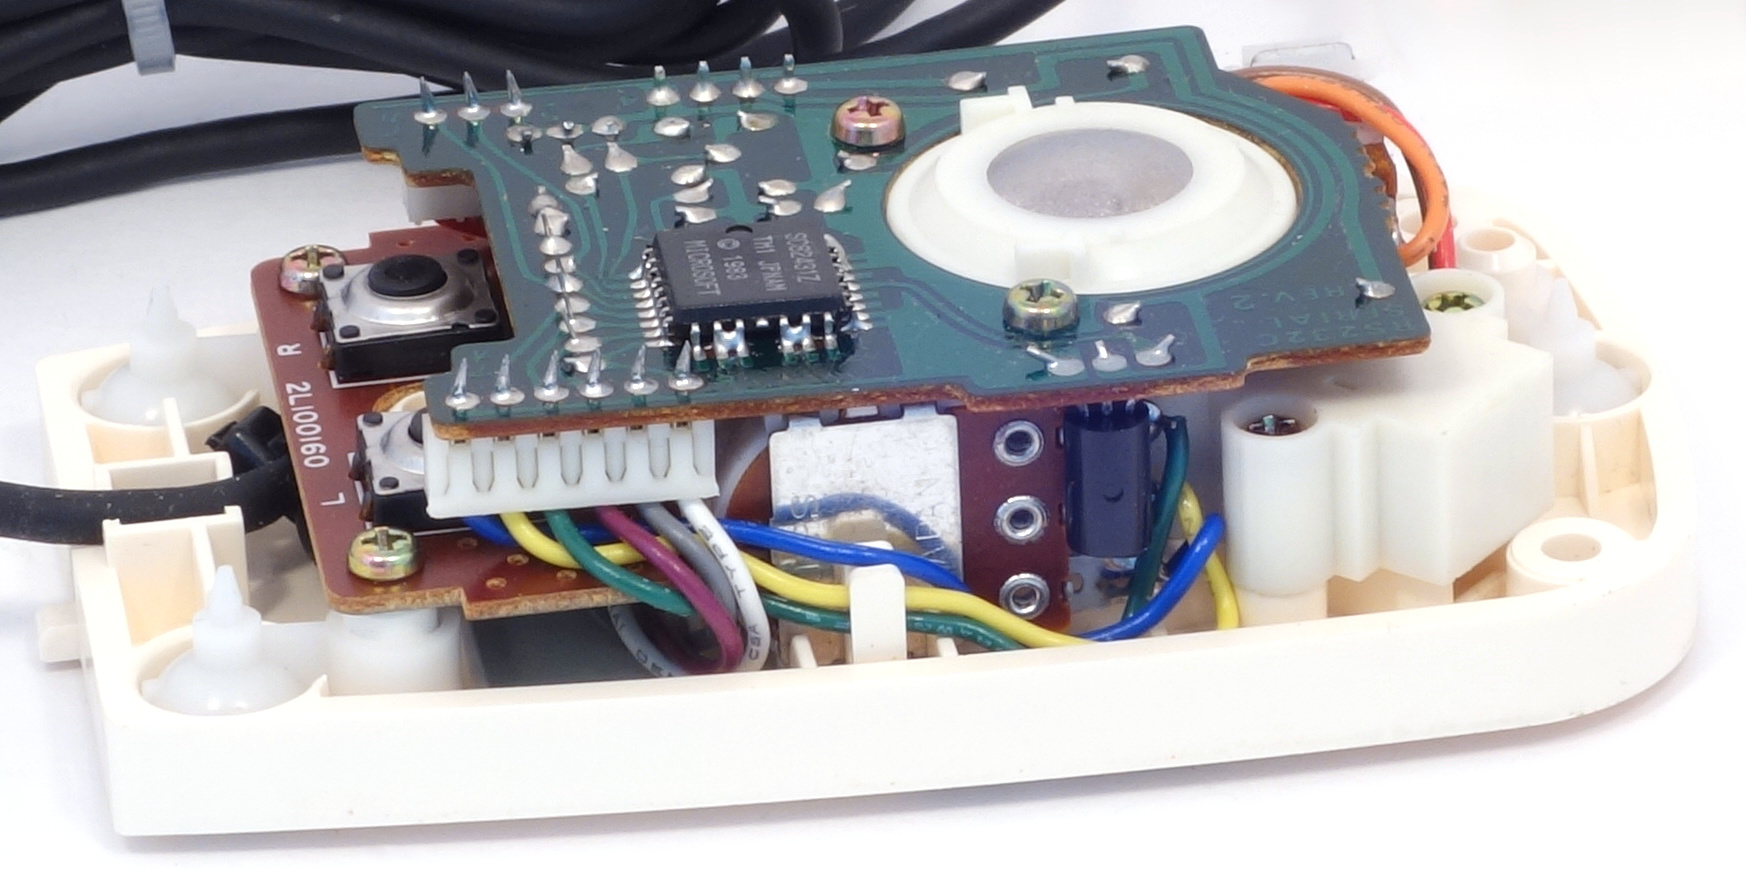
\includegraphics[scale=1]{1983_microsoft_green_eyed_mouse/inside_30.jpg}
    \caption{Microsoft Green Eyed Mouse disassembled}
    \label{fig:MicrosoftGreenEyedInside}
\end{figure}

\begin{thebibliography}{9}
\bibitem{mouses} Microsoft Green Eyed Mouse \url{https://web.archive.org/web/20211205011010/https://www.oldmouse.com/mouse/microsoft/greeneyed.shtml}
\bibitem{review} Hart G. Building a better mouse interface // PC Magazine, February 25, 1986. -- pp. 167-170. \url{https://archive.org/details/PC-Mag-1986-02-25/page/173/mode/2up}
\end{thebibliography}
\end{document}
